\documentclass[12pt,a4paper,oneside]{report}

% --- Pakiety podstawowe ---
\usepackage[utf8]{inputenc}
\usepackage[T1]{fontenc}
\usepackage[polish]{babel}
\usepackage{indentfirst} 
\usepackage{lmodern} % Lepsze czcionki Latin Modern

% --- Matematyka i~symbole ---
\usepackage{amsmath, amsfonts, amssymb, amsthm}

% --- Grafika i~tabele ---
\usepackage{graphicx}
\usepackage{booktabs}
\usepackage{array}
\usepackage{caption}
\usepackage{subcaption}
\usepackage{float}
\usepackage{xcolor}
\usepackage{tabularx}

% --- Kod źródłowy ---
\usepackage{listings}

% --- Bibliografia i~linki ---
\usepackage[numbers,sort&compress]{natbib}

% --- Ustawienia marginesów i~układu strony ---
\usepackage[top=2.5cm, bottom=2.5cm, left=3.5cm, right=2.5cm, headheight=16pt]{geometry}
\usepackage{fancyhdr}
\usepackage{titlesec}

% --- Konfiguracja nagłówków i~stopek ---
\pagestyle{fancy}
\fancyhf{}
\fancyhead[R]{\thepage}
\fancyhead[L]{\leftmark}
\renewcommand{\headrulewidth}{0.4pt}
\renewcommand{\chaptermark}[1]{\markboth{\thechapter.\ #1}{}}

% --- Konfiguracja tytułów rozdziałów ---
\titleformat{\chapter}[display]
 {\normalfont\huge\bfseries\color{darkgray}}
 {\chaptertitlename~\thechapter}{20pt}{\Huge}

% --- Interlinia i~skład ---
\usepackage{setspace}
\onehalfspacing
\sloppy % Pomaga przy overfull hbox w~języku polskim
% --- Definicje kolorów ---
\definecolor{darkgray}{rgb}{0.2,0.2,0.2}

\usepackage{microtype} % Poprawia skład i~kerning
\usepackage[hidelinks]{hyperref}

% --- Dane o~pracy ---
\title{Automatyczna segmentacja obrazu OCT siatkówki oka ludzkiego z~wykorzystaniem głębokiego uczenia maszynowego}
\author{Maksymilian Naskręt i~Eryk Naumienko}
\date{2026}

\begin{document}

% --- Strona tytułowa ---
\begin{titlepage}
 \begin{center}
 \vspace*{1cm}
 
 \textsc{\Large Politechnika Poznańska}\\[0.5cm]
 \textsc{\large Wydział Automatyki, Robotyki i~Elektrotechniki}\\[1.5cm]

 \vspace{1.5cm}

 {\huge \bfseries Automatyczna segmentacja obrazu OCT siatkówki oka ludzkiego z~wykorzystaniem głębokiego uczenia maszynowego}\\[2cm]

 \begin{minipage}{0.4\textwidth}
 \begin{flushleft} \large
 \emph{Autorzy:}\\
 Maksymilian \textsc{Naskręt}\\
 Eryk \textsc{Naumienko}
 \end{flushleft}
 \end{minipage}
 \begin{minipage}{0.4\textwidth}
 \begin{flushright} \large
 \emph{Promotor:} \\
 dr~inż.~Agnieszka \textsc{Stankiewicz}
 \end{flushright}
 \end{minipage}

 \vfill

 {\large Poznań, 2026}
 \end{center}
\end{titlepage}

\tableofcontents
\listoffigures
\listoftables

\chapter{Wstęp}

\section{Motywacja i~znaczenie kliniczne}

Współczesna okulistyka w~znacznym stopniu opiera się na zaawansowanych technikach obrazowania, wśród których Optyczna Koherentna Tomografia (ang.~\textit{Optical Coherence Tomography}, OCT) odgrywa kluczową rolę. Dzięki wysokiej rozdzielczości i~nieinwazyjności, OCT stało się standardem w~diagnostyce schorzeń siatkówki, takich jak zwyrodnienie plamki związane z~wiekiem (AMD) czy cukrzycowy obrzęk plamki (ang.~\textit{Diabetic Macular Edema}, DME). Jednym z~najistotniejszych wskaźników postępu choroby oraz skuteczności terapii jest obecność i~wielkość patologicznych przestrzeni płynowych: płynu wewnątrzsiatkówkowego (ang.~\textit{Intraretinal Fluid}, IRF), podsiatkówkowego (ang.~\textit{Subretinal Fluid}, SRF) oraz odwarstwień nabłonka barwnikowego siatkówki (ang.~\textit{Pigment Epithelium Detachment}, PED). Ręczna segmentacja tych zmian przez klinicystów jest procesem niezwykle pracochłonnym, subiektywnym i~podatnym na błędy, co stwarza pilną potrzebę opracowania precyzyjnych narzędzi automatycznych~\cite{retouch2019}.

\section{Problem badawczy}

Przez ostatnią dekadę w~dziedzinie segmentacji obrazów medycznych dominowały Konwolucyjne Sieci Neuronowe (CNN), a~architektura nnU-Net stała się referencyjnym punktem odniesienia (ang.~\textit{baseline}) dla wielu zadań analitycznych~\cite{isensee2021nnu}. Mimo sprawdzonych rezultatów empirycznych, sieci konwolucyjne posiadają strukturalne ograniczenia w~modelowaniu globalnych zależności kontekstowych ze względu na lokalny charakter operacji splotu. Odpowiedzią na te braki są architektury oparte na mechanizmie uwagi (ang.~\textit{Self-Attention}), znane jako Transformery, które po sukcesach w~przetwarzaniu języka naturalnego znajdują coraz szersze zastosowanie w~obszarze wizji komputerowej (\textit{Vision Transformers})~\cite{dosovitskiy2020vit}. Głównym problemem badawczym niniejszej pracy jest weryfikacja, czy i~w~jakim stopniu nowoczesne architektury transformerowe, takie jak SegFormer czy SwinUNETR, są w~stanie przewyższyć klasyczne podejścia konwolucyjne w~wymagającym zadaniu wieloklasowej segmentacji patologicznych przestrzeni płynowych w~obrazach OCT.\@

\section{Cel i~zakres pracy}

Głównym celem pracy jest opracowanie, implementacja i~przeprowadzenie systematycznego porównania skuteczności wybranych architektur głębokiego uczenia w~zadaniu automatycznej segmentacji obszarów IRF, SRF oraz PED na skanach OCT.\@ 

Zakres pracy obejmuje:
\begin{itemize}
 \item Przygotowanie i~wstępne przetwarzanie (ang.~\textit{preprocessing}) danych ze standaryzowanego, publicznego zbioru RETOUCH.\@
 \item Implementację i~wyuczenie modelu bazowego nnU-Net w~celu ustalenia poziomu referencyjnego.
 \item Adaptację oraz strojenie (ang.~\textit{fine-tuning}) zaawansowanych modeli transformerowych: SegFormer oraz SwinUNETR.\@
 \item Przeprowadzenie ewaluacji ilościowej z~wykorzystaniem metryk oceniających stopień pokrycia obszarów (Dice Score, mIoU) oraz dokładność wyznaczenia konturów (95.\ percentyl dystansu Hausdorffa~--- HD95).
 \item Analizę jakościową wyników, w~tym ekstrakcję i~wizualizację map uwagi (ang.~\textit{attention maps}) w~celu oceny interpretowalności decyzji podejmowanych przez sieci oparte na architekturze Transformer.
\end{itemize}

\section{Struktura pracy}

Praca została podzielona na siedem rozdziałów. Rozdział drugi przybliża podstawy teoretyczne obrazowania OCT oraz ewolucję metod segmentacji w~medycynie. W~rozdziale trzecim opisano wykorzystany zbiór danych oraz rygorystyczny proces jego przygotowania. Rozdział czwarty szczegółowo omawia wybrane architektury sieciowe oraz parametryzację i~metodologię badań. Wyniki eksperymentów wraz z~ich wizualizacją przedstawiono w~rozdziale piątym. Rozdział szósty zawiera analizę jakościową, analizę błędów oraz dyskusję otrzymanych rezultatów w~szerszym kontekście klinicznym. Pracę kończy rozdział siódmy, stanowiący podsumowanie osiągniętych rezultatów i~nakreślenie perspektyw na dalsze badania.

\chapter{Podstawy teoretyczne}

\section{Optyczna Koherentna Tomografia (OCT) siatkówki}

Optyczna Koherentna Tomografia (OCT) jest nieinwazyjną techniką obrazowania medycznego, która umożliwia uzyskiwanie przekrojowych obrazów struktur biologicznych z~mikrometryczną rozdzielczością~\cite{huang1991oct}. Zasada działania OCT opiera się na interferometrii niskokoherencyjnej, najczęściej w~konfiguracji interferometru Michelsona. Światło z~superluminescencyjnej diody (SLD) jest dzielone na dwie wiązki: referencyjną oraz pomiarową, która oświetla tkankę. Światło odbite od poszczególnych warstw siatkówki interferuje ze światłem z~ramienia referencyjnego, co pozwala na precyzyjny pomiar głębokości (A-scan). Poprzez skanowanie poprzeczne wiązki uzyskuje się dwuwymiarowe przekroje (B-scany), a~w~nowoczesnych urządzeniach typu Spectral-Domain (SD-OCT) możliwe jest generowanie pełnych rekonstrukcji trójwymiarowe.

\section{Patologie płynowe w~schorzeniach siatkówki}

W~przebiegu schorzeń objawiających się obrzękiem plamki, takich jak neowaskularna postać zwyrodnienia plamki związanego z~wiekiem (nAMD) oraz cukrzycowy obrzęk plamki (DME), dochodzi do patologicznego gromadzenia się płynów. W~literaturze i~praktyce klinicznej wyróżnia się trzy główne typy patologii podlegające segmentacji~\cite{retouch2019}:
\begin{enumerate}
 \item \textbf{Płyn wewnątrzsiatkówkowy (ang.~\textit{Intraretinal Fluid}, IRF):} gromadzi się wewnątrz warstw siatkówki neurosensorycznej, często tworząc charakterystyczne przestrzenie cystoidalne.
 \item \textbf{Płyn podsiatkówkowy (ang.~\textit{Subretinal Fluid}, SRF):} gromadzi się pomiędzy warstwą fotoreceptorów a~nabłonkiem barwnikowym siatkówki (ang.~\textit{Retinal Pigment Epithelium}, RPE).
 \item \textbf{Odwarstwienie nabłonka barwnikowego (ang.~\textit{Pigment Epithelium Detachment}, PED):} uniesienie warstwy RPE nad błonę Brucha, często wypełnione płynem surowiczym, krwią lub tkanką włóknisto-naczyniową.
\end{enumerate}
Precyzyjne monitorowanie objętości tych przestrzeni jest kluczowe dla oceny progresji choroby oraz personalizacji terapii inhibitorami VEGF.\@

\section{Segmentacja semantyczna w~obrazowaniu medycznym}

Segmentacja semantyczna polega na przypisaniu każdemu elementowi obrazu (pikselowi lub wokselowi) etykiety przynależności do określonej klasy anatomicznej lub patologicznej. W~kontekście OCT, zadanie to wymaga wyznaczenia precyzyjnych granic obszarów płynowych. Do głównych wyzwań analitycznych należą: niski stosunek sygnału do szumu (obecność szumu typu \textit{speckle}), artefakty cieniowania (ang.~\textit{shadowing}) oraz znaczna zmienność morfologiczna struktur dotkniętych zaawansowanym procesem chorobowym.

\section{Konwolucyjne Sieci Neuronowe (CNN)}

Przełomem w~automatycznej analizie obrazów medycznych było wprowadzenie głębokich konwolucyjnych sieci neuronowych. Architektury te wykorzystują operację splotu do automatycznej i~hierarchicznej ekstrakcji cech. Kluczową zaletą CNN jest wbudowane indukcyjne skrzywienie (ang.~\textit{inductive bias}) w~postaci niezmienniczości translacyjnej oraz lokalności, co pozwala na efektywne uczenie przy ograniczonej liczbie próbek. Standardem w~segmentacji medycznej stała się architektura \textit{U-Net}, oparta na symetrycznej strukturze kodująco-dekodującej z~połączeniami skrótowymi (\textit{skip connections}), które umożliwiają agregację cech o~wysokiej rozdzielczości przestrzennej z~głębokimi cechami semantycznymi~\cite{ronneberger2015unet}. Ewolucją tego podejścia jest system nnU-Net, który automatyzuje proces konfiguracji sieci, dostosowując ją do specyfiki danego zbioru danych~\cite{isensee2021nnu}.

\begin{figure}[htbp]
    \centering
    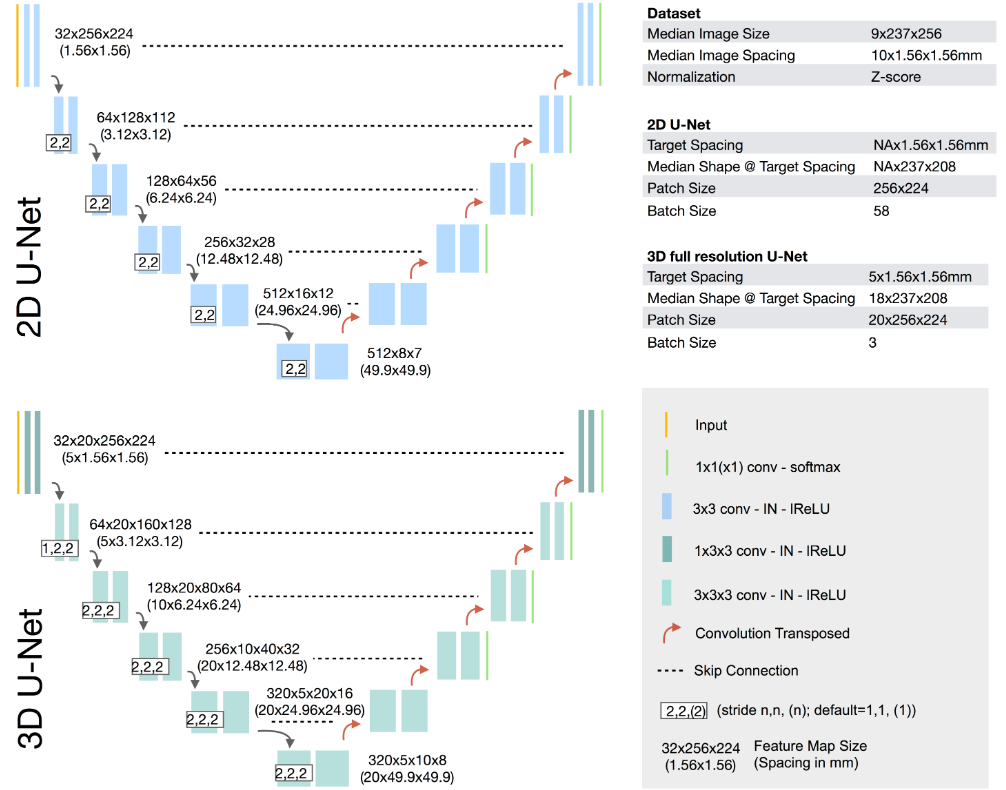
\includegraphics[width=0.85\textwidth]{unet-schema.png}
    \caption{Architektura sieci U-Net: widoczna symetryczna struktura ścieżki kontrastującej (enkoder) i~rozszerzającej (dekoder) połączonych połączeniami skrótowymi (opracowanie własne na podstawie~\cite{nnunet_medium}).}
    \label{fig:unet_schema}
\end{figure}

\section{Transformery w~wizji komputerowej}

Mimo sukcesów CNN, ich podstawowa operacja splotu ogranicza pole widzenia (ang.~\textit{receptive field}) do lokalnego sąsiedztwa pikseli. Modelowanie globalnych zależności kontekstowych wymaga w~takim przypadku stosowania bardzo głębokich struktur. Vision Transformers (ViT) eliminują to ograniczenie poprzez mechanizm samo-uwagi (ang.~\textit{self-attention}), pozwalający na analizę relacji między wszystkimi fragmentami obrazu jednocześnie~\cite{dosovitskiy2020vit}. W~segmentacji medycznej podejście to zaowocowało architekturami takimi jak SwinUNETR, wykorzystującymi hierarchiczne Transformery z~przesuwnymi oknami (ang.~\textit{shifted windows}) w~celu redukcji złożoności obliczeniowej~\cite{hatamizadeh2022swinunetr}, oraz SegFormer, który łączy hierarchiczny enkoder transformerowy z~wydajnym dekoderem MLP (\textit{Multi-Layer Perceptron}). Dekoder ten agreguje wieloskalowe cechy z~różnych etapów enkodera, co pozwala na skuteczne łączenie informacji o~wysokiej rozdzielczości z~głębokim kontekstem semantycznym, przy jednoczesnym wyeliminowaniu potrzeby stosowania pozycjonowania absolutnego~\cite{xie2021segformer}. Szczegółowy schemat blokowy architektury SegFormer, ilustrujący hierarchiczną strukturę enkodera oraz sposób agregacji cech w~dekoderze MLP, przedstawiono na rysunku~\ref{fig:segformer_schema}.

\begin{figure}[htbp]
    \centering
    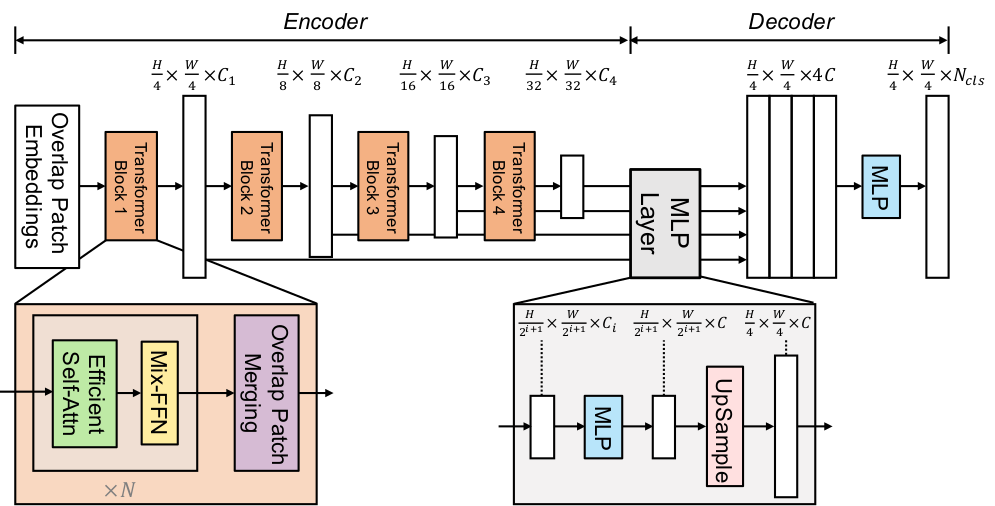
\includegraphics[width=0.9\textwidth]{segformer-schema.png}
    \caption{Schemat architektury SegFormer: hierarchiczny enkoder transformerowy generujący wieloskalowe mapy cech oraz dekoder MLP agregujący informacje z~różnych poziomów rozdzielczości (opracowanie własne na podstawie~\cite{hfsegformer}).}
\label{fig:segformer_schema}
\end{figure}

\chapter{Zbiór danych i~wstępne przetwarzanie}

\section{Charakterystyka zbioru danych RETOUCH}

W~pracy wykorzystano publicznie dostępny zbiór danych RETOUCH, przygotowany na potrzeby wyzwania \textit{Retinal Macular Lesion Segmentation Challenge} zorganizowanego podczas konferencji MICCAI 2017~\cite{retouch2019}. Zbiór ten charakteryzuje się wysokim stopniem heterogeniczności, gdyż zawiera skany OCT pacjentów z~rozpoznanym zwyrodnieniem plamki związanym z~wiekiem (AMD) oraz zakrzepem żyły środkowej siatkówki (RVO), zarejestrowane przy użyciu trzech różnych urządzeń klinicznych: Cirrus, Spectralis oraz Topcon. Zróżnicowanie parametrów technicznych oraz statystyki intensywności obrazów dla poszczególnych producentów zestawiono w~tabeli~\ref{tab:dataset_stats}.

\begin{table}[htbp]
    \centering
    \caption{Statystyki zbioru RETOUCH w~podziale na producentów urządzeń. Rozdzielczość podano w~formacie: szerokość $\times$ liczba przekrojów $\times$ wysokość.}
\label{tab:dataset_stats}
    \begin{tabularx}{\textwidth}{lXccc}
        \toprule
        Urządzenie & Rozdzielczość [px] & Średnia jasność & Odchylenie std. & Liczba B-skanów \\
        \midrule
        Cirrus & $512 \times 128 \times 1024$ & 66,63 & 48,05 & 3072 \\
        Spectralis & $496 \times 49 \times 512$ & 74,54 & 45,78 & 1176 \\
        Topcon & $885 \times 128 \times 512$ & 75,05 & 47,13 & 2674 \\
        \bottomrule
    \end{tabularx}
\end{table}

Każdy wolumen OCT został opatrzony referencyjnymi maskami segmentacji (ang.~\textit{ground truth}), obejmującymi trzy klasy patologiczne: płyn wewnątrzsiatkówkowy (IRF), płyn podsiatkówkowy (SRF) oraz odwarstwienie nabłonka barwnikowego siatkówki (PED). Przykładową wizualizację przekroju z~oznaczonymi patologiami przedstawiono na rysunku~\ref{fig:pathology_examples}.

\begin{figure}[htbp]
    \centering
    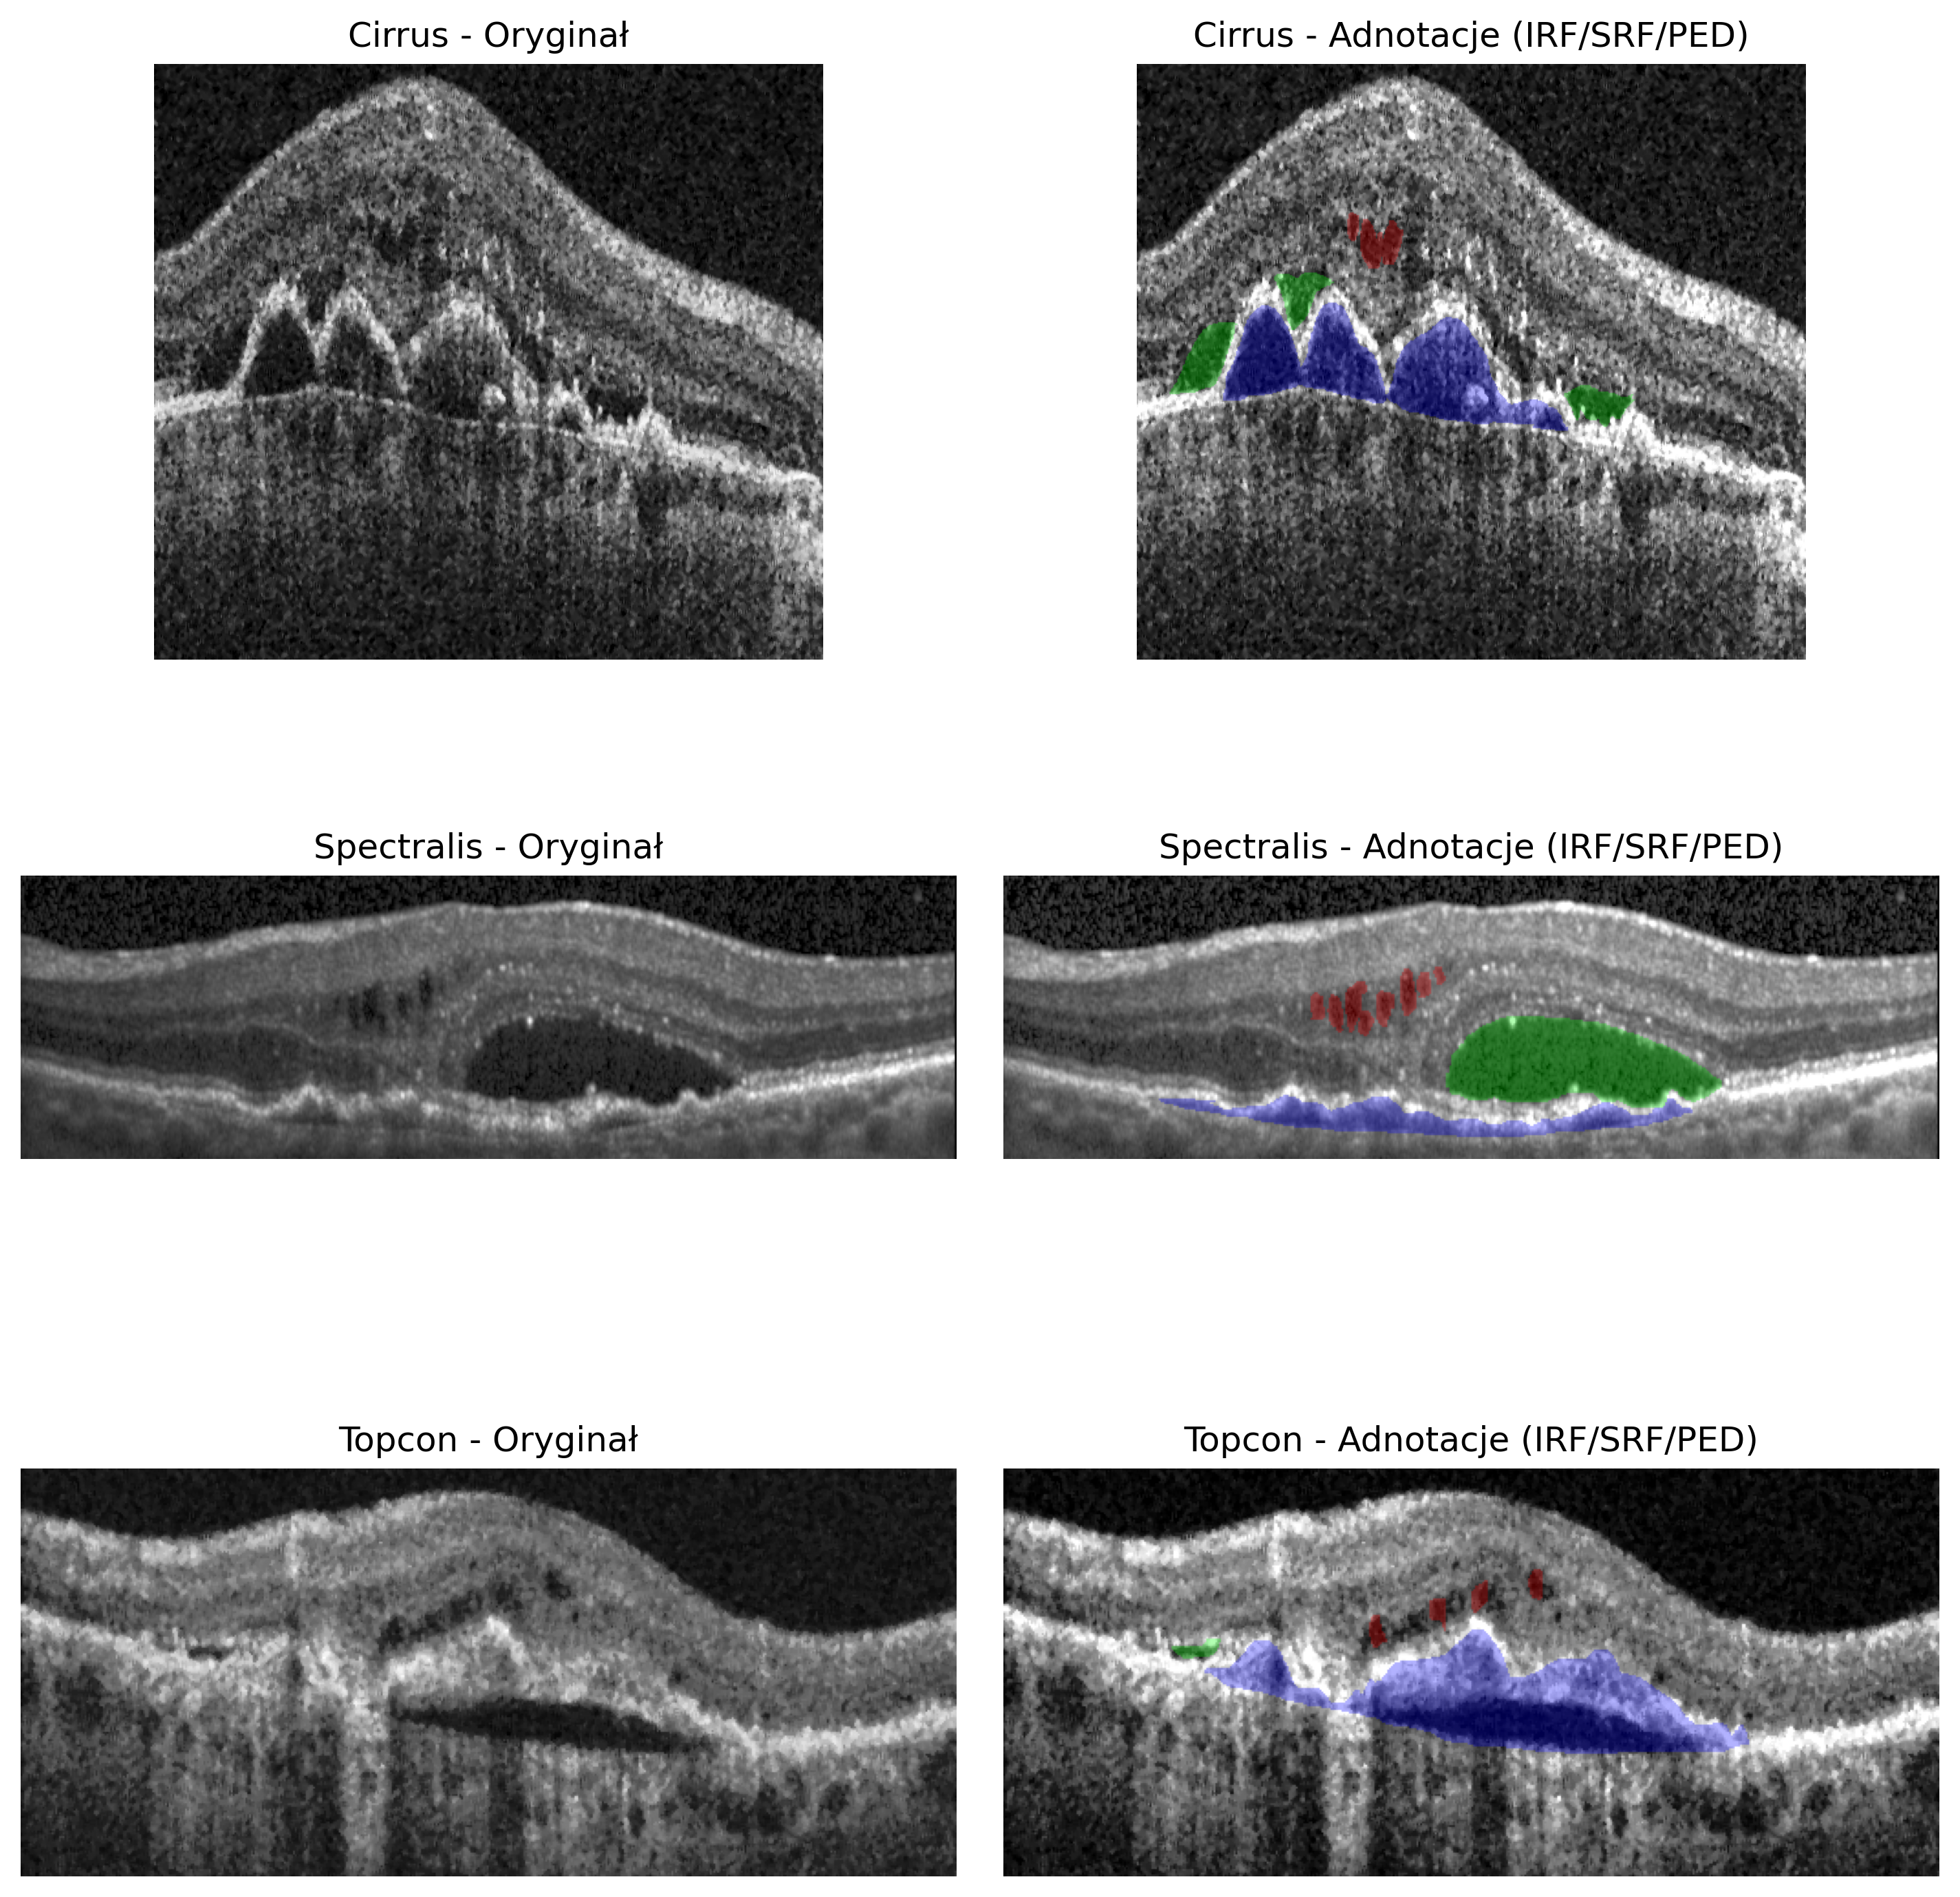
\includegraphics[width=0.9\textwidth]{pathology_examples.png}
    \caption{Przykładowy przekrój B-scan ze zbioru RETOUCH z~widocznymi patologiami: płyn wewnątrzsiatkówkowy (IRF, kolor czerwony), podsiatkówkowy (SRF, kolor zielony) oraz odwarstwienie nabłonka barwnikowego siatkówki (PED, kolor niebieski).}
\label{fig:pathology_examples}
\end{figure}

\section{Wyzwania związane z~heterogenicznością danych}

Głównym wyzwaniem analitycznym wynikającym z~wykorzystania zbioru RETOUCH jest znacząca rozpiętość charakterystyki obrazów. Różnice obejmują nie tylko rozdzielczość przestrzenną (Tabela~\ref{tab:dataset_stats}), ale przede wszystkim stosunek sygnału do szumu, kontrast tkanek oraz specyficzne dla danego urządzenia artefakty (np. cieniowanie naczyń). Aby umożliwić skuteczną generalizację modeli głębokiego uczenia, konieczne było wdrożenie ustandaryzowanego potoku przetwarzania danych.

\section{Proces przetwarzania danych i~implementacja klasy Dataset}

W~celu ujednolicenia danych wejściowych zaimplementowano autorski proces przetwarzania (ang.~\textit{preprocessing pipeline}), zintegrowany z~klasą \texttt{OCTDataset}. Kluczowe kroki przygotowania obrazów obejmują:

\begin{enumerate}
 \item \textbf{Podział na zbiory (Data Splitting):} Dane podzielono na zbiory treningowy, walidacyjny i~testowy na poziomie całych pacjentów (wolumenów OCT). Takie podejście zapobiega wyciekowi danych (ang.~\textit{data leakage}), co jest szczególnie istotne w~proponowanej metodzie 2.5D, gdzie sąsiednie przekroje tego samego pacjenta są silnie skorelowane.
 \item \textbf{Standaryzacja rozdzielczości:} Ze względu na różnice w~rozmiarach B-skanów pomiędzy producentami, wszystkie obrazy zostały przeskalowane do wspólnego wymiaru $512 \times 512$ pikseli przy użyciu interpolacji dwuliniowej (biblioteka \texttt{PIL}, metoda \texttt{Image.BILINEAR}).
 \item \textbf{Normalizacja kliniczna (Clipping):} W~celu redukcji wpływu ekstremalnych wartości szumu typu \textit{speckle}, zastosowano przycinanie intensywności (ang.~\textit{clipping}) do zakresu 1--99 percentyla rozkładu jasności, a~następnie wykonano normalizację liniową do przedziału $[0, 1]$. Metoda ta pozwala na zachowanie wysokiego kontrastu struktur anatomicznych przy jednoczesnym odfiltrowaniu artefaktów świecenia.
 \item \textbf{Podejście 2.5D (Kontekst przestrzenny):} Zastosowano strategię wielokanałowego wejścia, w~której dla każdego docelowego przekroju $t$ dołączane są sąsiednie slajdy $t-1$ oraz $t+1$. Wynikowy tensor wejściowy o~wymiarze $512 \times 512 \times 3$ dostarcza modelowi lokalnego kontekstu wolumetrycznego, co ułatwia odróżnienie szumu od rzeczywistych, ciągłych struktur płynowych (Rysunek~\ref{fig:logic_25d}).
 \item \textbf{Reprezentacja wielomodalna (Multimodal):} W~ramach eksperymentów z~modelami transformerowymi wykorzystano rozszerzony zestaw cech wejściowych. Oprócz oryginalnego B-skanu, do sieci podawane są mapy krawędzi oraz obrazy odszumione. Taka reprezentacja wspomaga mechanizm uwagi w~lokalizacji subtelnych granic patologii.
\end{enumerate}

\begin{figure}[htbp]
    \centering
    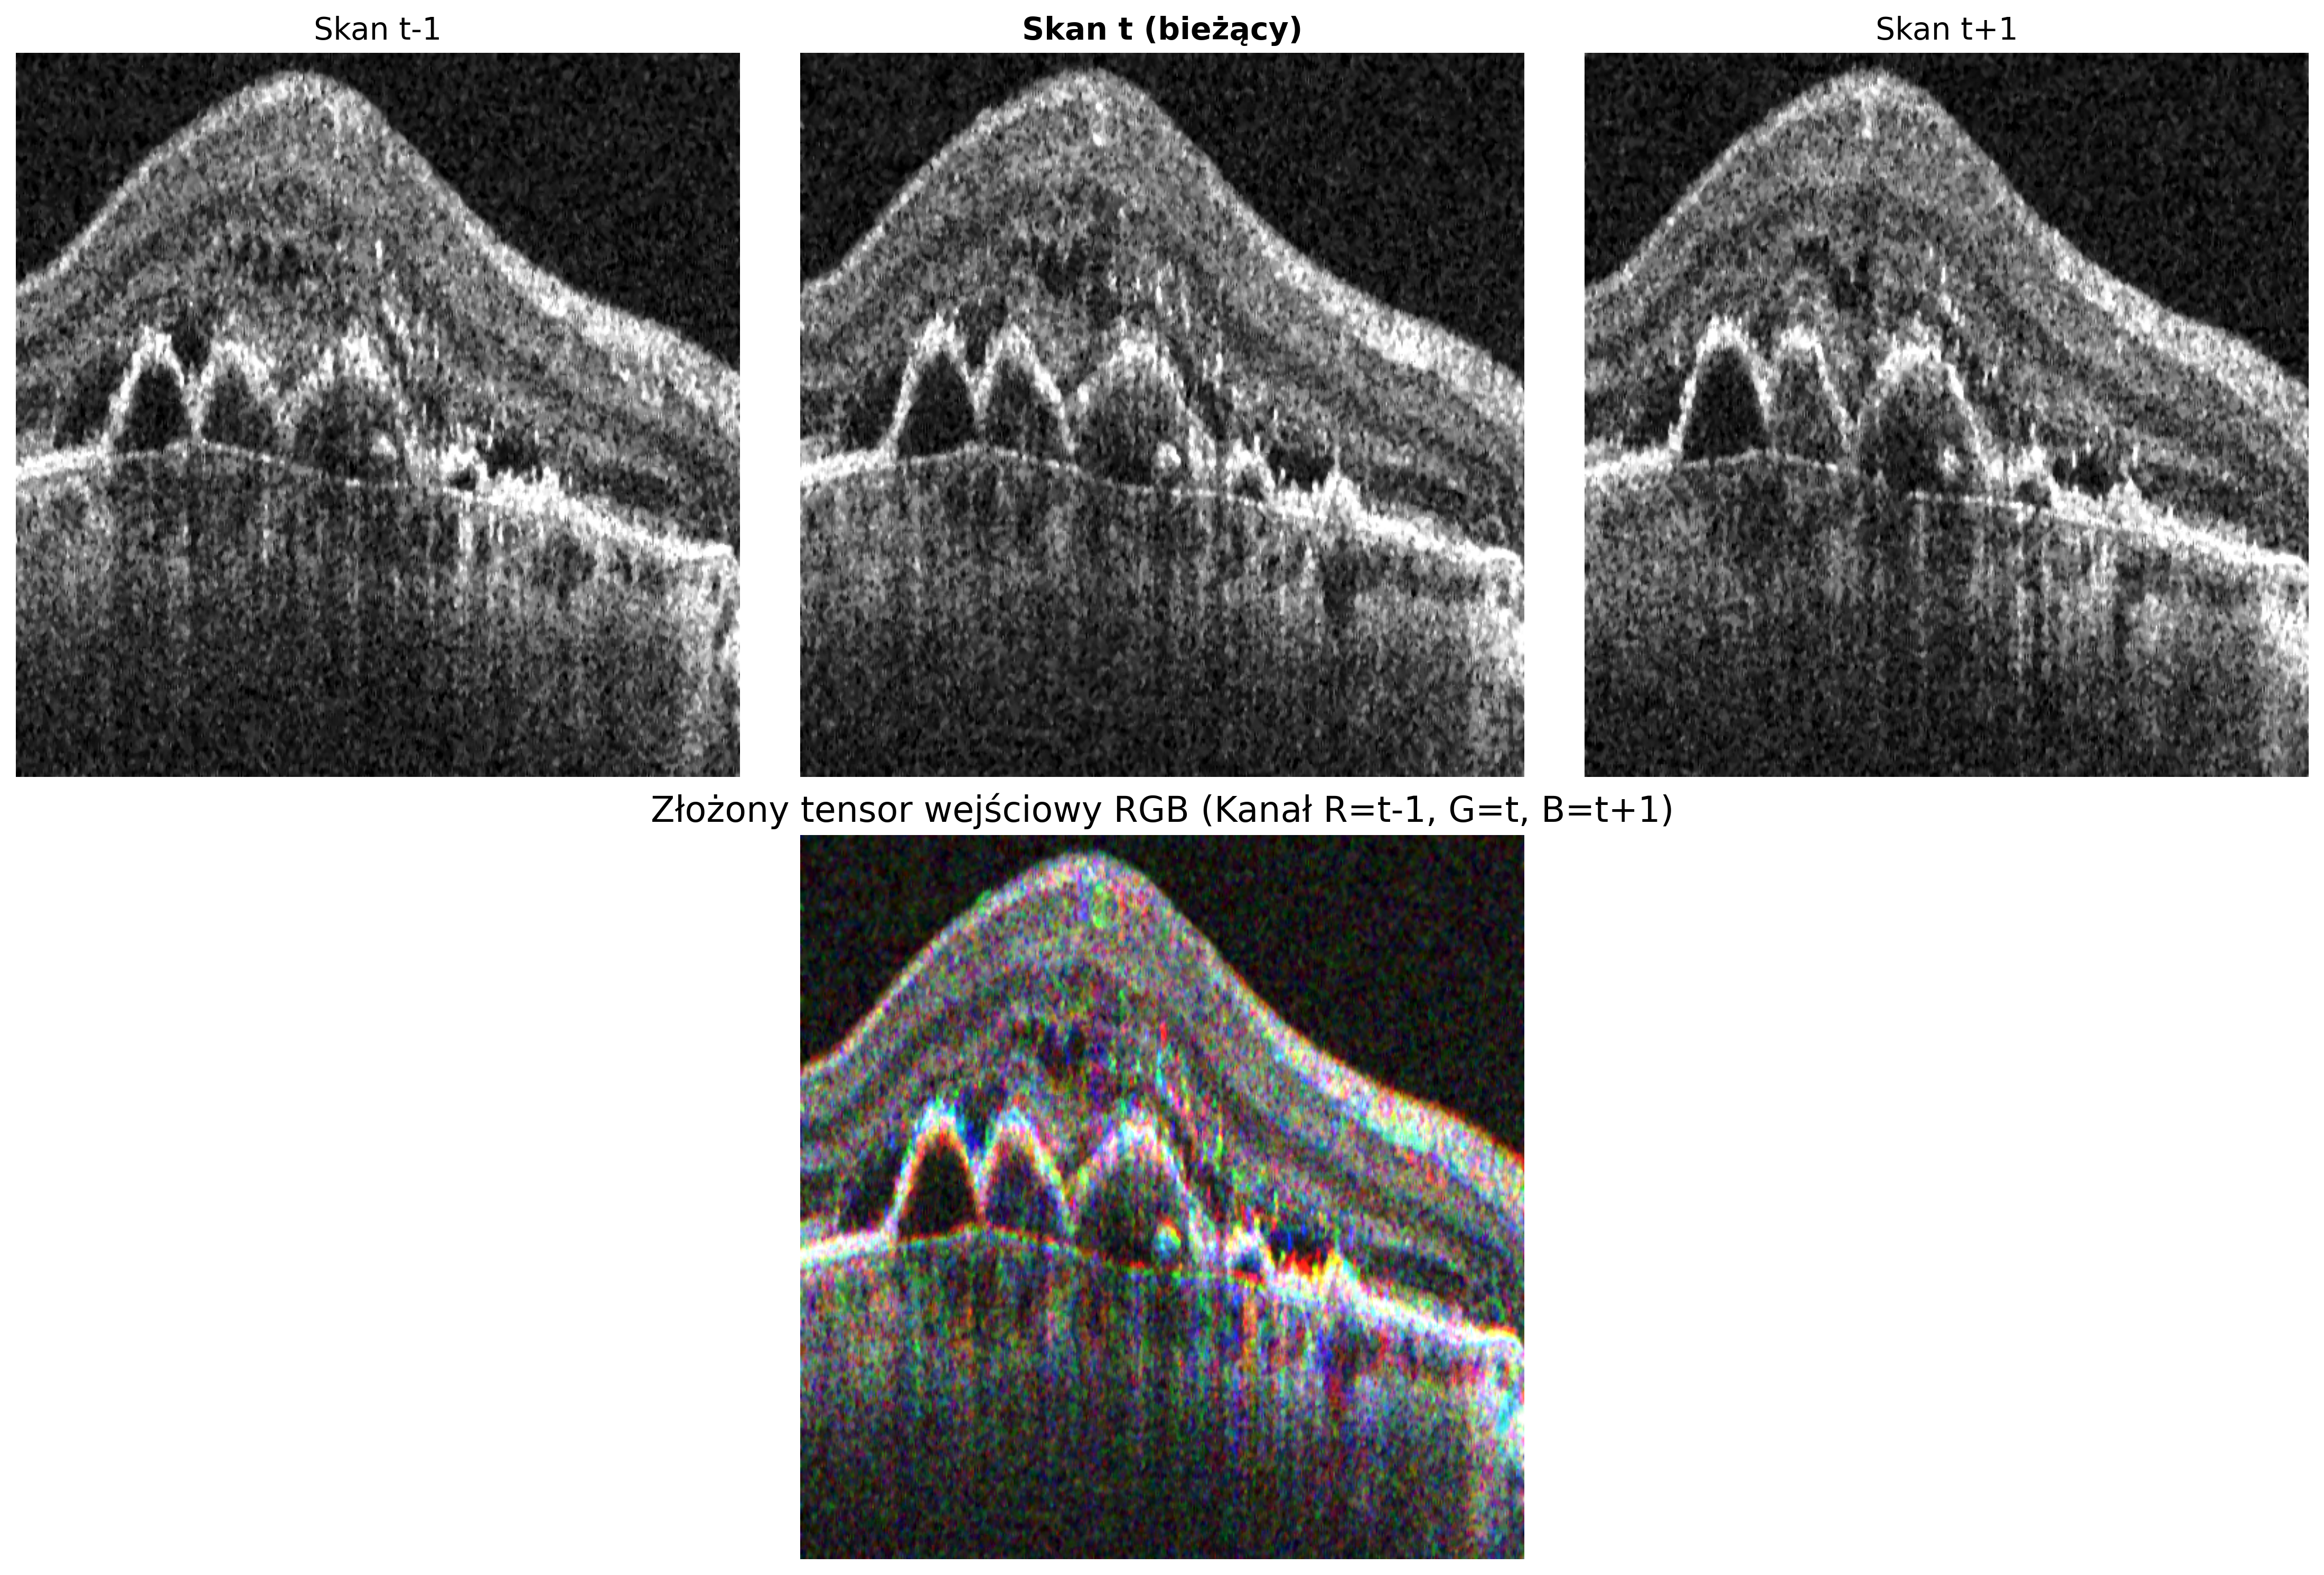
\includegraphics[width=\textwidth]{logic_25d.png}
    \caption{Wizualizacja logiki 2.5D: tensor wejściowy tworzony przez bieżący B-scan (kanał zielony) oraz bezpośrednio sąsiadujące z~nim przekroje OCT: poprzedni (kanał czerwony) i~następny (kanał niebieski).}
\label{fig:logic_25d}
\end{figure}

\chapter{Metodologia}

\section{Architektura bazowa (Baseline): nnU-Net}

Jako punkt odniesienia (baseline) w~niniejszej pracy wykorzystano system nnU-Net (\textit{no-new-Net}). Jest to framework, który automatyzuje proces konfiguracji sieci neuronowej do segmentacji obrazów medycznych~\cite{isensee2021nnu}. nnU-Net nie wprowadza nowej architektury, lecz optymalizuje klasycznego U-Neta poprzez automatyczny dobór hiperparametrów, takich jak rozmiar paczek (\textit{batch size}), planowanie szybkości uczenia (\textit{learning rate schedule}) oraz techniki augmentacji, bazując na właściwościach zbioru danych (tzw. \textit{dataset fingerprint}). W~eksperymentach wykorzystano konfigurację 2D, aby rzetelnie porównać wyniki z~nowszymi modelami transformerowymi.

\section{Implementowane architektury U-Net}

\subsection{U-Net z enkoderem ResNet34}

W ramach pracy zaimplementowano model U-Net z enkoderem ResNet34, stanowiący klasyczne podejście konwolucyjne do segmentacji semantycznej obrazów medycznych. Architektura U-Net została pierwotnie zaproponowana z myślą o segmentacji obrazów biomedycznych i charakteryzuje się symetryczną strukturą enkodera oraz dekodera połączonych ścieżkami skrótowymi~\cite{ronneberger2015unet}. W implementowanym wariancie część kodująca została zastąpiona siecią ResNet34, wykorzystującą połączenia rezydualne ułatwiające uczenie głębszych modeli~\cite{he2016deep}.

Model ten charakteryzuje się następującymi cechami:
\begin{itemize}
    \item \textbf{Enkoder ResNet34:} zastosowanie sieci ResNet34 pozwala wykorzystać cechy niskiego poziomu, takie jak krawędzie, tekstury i lokalne kontrasty, które mogą być przydatne również w analizie obrazów OCT.
    \item \textbf{Połączenia skrótowe U-Net:} przekazywanie cech z enkodera do dekodera umożliwia zachowanie informacji przestrzennej, istotnej dla precyzyjnego wyznaczania granic obszarów IRF, SRF oraz PED.
    \item \textbf{Wstępnie wytrenowane wagi:} wykorzystanie wag wytrenowanych na zbiorze ImageNet pozwala rozpocząć uczenie od bardziej stabilnej reprezentacji cech, zamiast trenować cały model od podstaw.
\end{itemize}

\subsection{Attention U-Net}

Drugim zaimplementowanym wariantem był Attention U-Net, czyli rozszerzenie klasycznej architektury U-Net o mechanizmy bramek uwagi~\cite{oktay2018attention}. Model ten zachowuje strukturę enkoder-dekoder, jednak informacje przekazywane przez połączenia skrótowe są dodatkowo filtrowane. Dzięki temu dekoder otrzymuje przede wszystkim te cechy, które są istotne dla lokalizacji segmentowanych struktur.

Architektura Attention U-Net charakteryzuje się następującymi elementami:
\begin{itemize}
    \item \textbf{Bramki uwagi:} moduły attention gate uczą się wzmacniać obszary istotne dla segmentacji oraz tłumić informacje pochodzące z tła lub artefaktów obrazu.
    \item \textbf{Selektywne połączenia skrótowe:} w odróżnieniu od klasycznego U-Neta, cechy z enkodera nie są przekazywane bezpośrednio, lecz podlegają filtracji zależnej od kontekstu dekodera.
    \item \textbf{Zastosowanie w segmentacji drobnych zmian:} mechanizm uwagi jest szczególnie przydatny w obrazach OCT, gdzie niewielkie cysty IRF mogą zajmować małą część obrazu i być trudne do odróżnienia od szumu oraz struktur anatomicznych.
\end{itemize}

\section{Modele transformerowe}

\subsection{SegFormer}

SegFormer to wydajna architektura transformerowa zaprojektowana specjalnie do segmentacji semantycznej~\cite{xie2021segformer}. Charakteryzuje się ona hierarchicznym enkoderem oraz lekkim dekoderem MLP, co pozwala na skuteczne modelowanie globalne przy zachowaniu wydajności (Rysunek~\ref{fig:segformer_schema_v2}).

\begin{figure}[htbp]
    \centering
    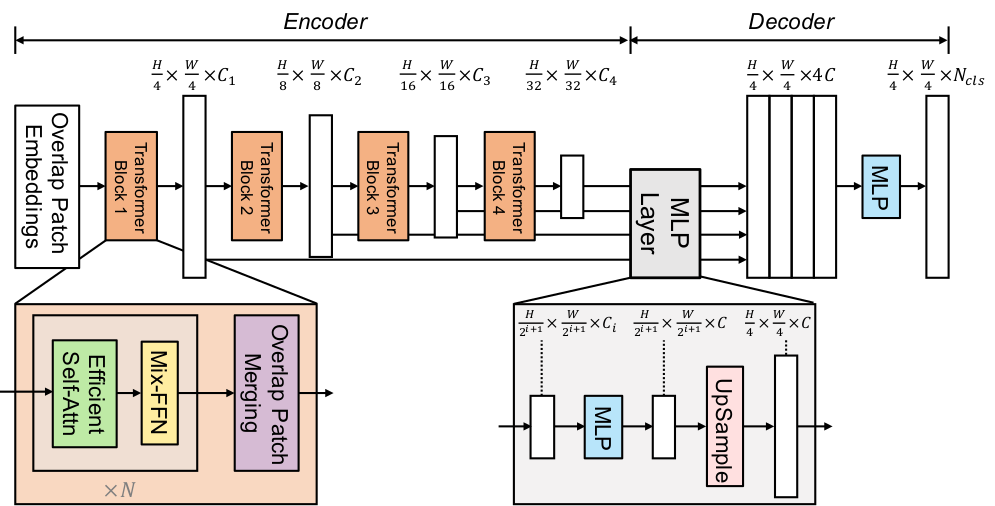
\includegraphics[width=0.85\textwidth]{segformer-schema.png}
    \caption{Szczegółowa architektura modelu SegFormer wykorzystana w~procesie segmentacji patologii OCT.\@ Widoczna hierarchiczna struktura enkodera MiT oraz proces agregacji cech w~dekoderze MLP (na podstawie~\cite{hfsegformer}).}
\label{fig:segformer_schema_v2}
\end{figure}

\subsection{SwinUNETR i~modele bazowe}

SwinUNETR (\textit{Swin Transformer-based Hierarchical Neural Network for Biomedical Image Segmentation}) to architektura łącząca potęgę Transformerów i~struktury U-Net, dedykowana danym medycznym~\cite{hatamizadeh2022swinunetr}. Pełna walidacja i optymalizacja modelu SwinUNETR ze względu na wysokie wymagania obliczeniowe oraz konieczność zastosowania technik uczenia na większych wolumenach danych, wykracza poza ramy niniejszego raportu i stanowi kierunek dalszych prac. Punktem odniesienia w~pracy pozostaje model nnU-Net.

\section{Strategia uczenia i~optymalizacja}

\subsection{Uczenie modeli konwolucyjnych (CNN)} 
Modele z~rodziny U-Net trenowano z~wykorzystaniem optymalizatora AdamW oraz harmonogramu szybkości uczenia \textit{CosineAnnealingLR}. Początkową szybkość uczenia (\textit{learning rate}) ustalono na poziomie $1 \times 10^{-4}$. W~procesie uczenia wykorzystano augmentacje z~biblioteki \textit{Albumentations}, obejmujące: rotacje ($\pm 15^\circ$), odbicia lustrzane, losowe zmiany jasności oraz dodanie szumu gaussowskiego ($\sigma_{max}=0.05$). Wykorzystanie wag wstępnie wytrenowanych na zbiorze ImageNet pozwoliło na szybszą zbieżność modeli mimo specyfiki obrazowania medycznego.

\subsection{Uczenie modeli transformerowych} 
Ze względu na większą złożoność obliczeniową architektur SegFormer oraz SwinUNETR, zastosowano optymalizator AdamW z~niższą szybkością uczenia $5 \times 10^{-5}$ oraz zanikaniem wag (\textit{weight decay}) $5 \times 10^{-2}$. Wykorzystano technikę akumulacji gradientu (\textit{Gradient Accumulation}), aby uzyskać efektywny rozmiar paczki (\textit{effective batch size}) równy 32 przy ograniczonej pamięci VRAM (12~GB). Proces stabilizowano poprzez 15~epok rozgrzewki (\textit{warmup}), po których następowało wielomianowe zanikanie szybkości uczenia. W~celu optymalizacji wykorzystano automatyczną mieszaną precyzję (ang.~\textit{Automatic Mixed Precision}, AMP).

\section{Funkcje kosztu i~postprocessing}

\subsection{Hybrydowa funkcja kosztu dla modeli Transformer}
Ze względu na ekstremalne niezrównoważenie klas (tło stanowi $>98\%$ pikseli), zastosowano złożoną funkcję kosztu łączącą \textit{Focal Loss} oraz \textit{Tversky Loss}. 

\textbf{Focal Loss} (FL) jest zaawansowaną modyfikacją entropii krzyżowej, zaprojektowaną do redukcji wpływu łatwych przykładów (tła) na proces uczenia. Wprowadza ona czynnik modulujący $(1 - p_t)^\gamma$, który dynamicznie skaluje stratę:
\begin{equation}
    FL(p_t) = -\alpha_t (1 - p_t)^\gamma \log(p_t)
\end{equation}
gdzie $\gamma$ to parametr skupienia (\textit{focusing parameter}), przyjęty jako $3.0$ w~celu silnego wzmocnienia błędu dla rzadkich pikseli patologicznych, natomiast $\alpha_t$ to parametr balansujący wagę poszczególnych klas.

\textbf{Tversky Loss} (TL) stanowi uogólnienie współczynnika Dice'a, pozwalając na asymetryczne karanie błędów typu \textit{False Negative} (FN) oraz \textit{False Positive} (FP), co jest kluczowe w~diagnostyce medycznej:
\begin{equation}
    TL(p, \hat{y}) = \frac{\sum p_i \hat{y}_i}{\sum p_i \hat{y}_i + \alpha \sum p_i (1-\hat{y}_i) + \beta \sum (1-p_i) \hat{y}_i}
\end{equation}
W~niniejszej pracy zastosowano tryb \textit{Clinical High-Recall} ($\alpha=0.1, \beta=0.9$), co oznacza dziewięciokrotnie silniejsze karanie pominięcia patologii ($\beta$) niż błędnego wykrycia ($\alpha$).

\subsection{Klinicznie motywowany postprocessing}
W~fazie wnioskowania (ang.~\textit{inference}) dla modeli transformerowych wdrożono dedykowany moduł poprawy jakości segmentacji:
\begin{itemize}
 \item \textbf{Skalibrowane progi decyzyjne:} w~celu optymalizacji czułości klinicznej, progi prawdopodobieństwa zostały obniżone względem standardowej wartości 0.50. Dla klasy IRF przyjęto próg 0.30, natomiast dla klas SRF oraz PED wartość 0.40.
 \item \textbf{Separacja morfologiczna:} zastosowanie operacji otwarcia (\textit{opening}) w~celu rozdzielenia wizualnie połączonych struktur.
 \item \textbf{Filtracja powierzchniowa:} usuwanie izolowanych skupisk pikseli o~polu mniejszym niż 50~px.
 \item \textbf{Wyostrzanie konturów PED:} zastosowanie filtra wyostrzającego (\textit{Unsharp Mask}) w~celu lepszego odwzorowania nieregularnej morfologii PED.
\end{itemize}

\section{Wizualizacja mechanizmów uwagi (Attention Visualization)}

W~celu zapewnienia klinicznej interpretowalności modeli, zaimplementowano dedykowany moduł \texttt{attention\_visualizer.py}. Pozwala on na analizę procesu decyzyjnego poprzez ekstrakcję wag samo-uwagi (\textit{self-attention}) z~bloków transformerowych enkodera.

Proces wizualizacji obejmuje:
\begin{enumerate}
 \item \textbf{Ekstrakcja wag atencji:} wykorzystanie mechanizmu przechwytywania wag z~poszczególnych warstw. Na drodze analizy jakościowej ustalono, że najbardziej użyteczne klinicznie mapy pochodzą z~późniejszych warstw enkodera (\textbf{indeksy 6 lub 7}), gdzie model precyzyjnie zarysowuje granice strukturalne odwarstwień PED oraz obszarów SRF. Jednocześnie zaobserwowano, że dla drobnych zmian typu IRF mapy atencji na tych poziomach są mało informacyjne, co wynika z~rozbieżności pomiędzy skalą przestrzenną małych cyst a~szerokim polem widzenia głębokich warstw transformera.
 \item \textbf{Agregacja wielogłowicowa:} uśrednianie wag z~wielu głowic atencji w~celu uzyskania spójnej mapy aktywacji dla całego obrazu.
 \item \textbf{Interpolacja i~korekcja Gamma:} rzutowanie map na wymiar $512 \times 512$ oraz zastosowanie korekcji Gamma ($\gamma=0.5$), co znacząco zwiększyło kontrast wizualny najbardziej istotnych obszarów.
 \item \textbf{Analiza selektywna:} automatyczny wybór najbardziej reprezentatywnych przypadków klinicznych o~wysokim współczynniku IoU.
\end{enumerate}

\chapter{Wyniki eksperymentów}

\section{Metodyka ewaluacji i~metryki kliniczne}

W~celu rzetelnej oceny opracowanych modeli, zaimplementowano zestaw metryk ilościowych, pozwalających na ocenę stopnia pokrycia obszarów oraz precyzji wyznaczenia granic patologii.

\textbf{Dice Similarity Coefficient (DSC)} mierzy podobieństwo dwóch zbiorów pikseli i~jest definiowany jako:
\begin{equation}
    DSC(A, B) = \frac{2 |A \cap B|}{|A| + |B|}
\end{equation}

\textbf{Mean Intersection over Union (mIoU)} informuje o~średnim stopniu pokrycia masek predykcyjnych z~referencyjnymi dla wszystkich klas patologicznych:
\begin{equation}
    mIoU = \frac{1}{C} \sum_{c=1}^C \frac{|A_c \cap B_c|}{|A_c \cup B_c|}
\end{equation}
gdzie $C=3$ to liczba analizowanych klas płynów (IRF, SRF, PED).

Dodatkowo zastosowano metrykę odległościową \textit{Hausdorff Distance 95} (HD95), która informuje o~maksymalnym błędzie dopasowania konturów w~pikselach. Wykorzystanie 95.\ percentyla pozwala na uodpornienie metryki na pojedyncze, odizolowane błędy brzegowe, które mogłyby nienaturalnie zawyżyć wynik.

\section{Szczegółowa analiza wyników eksperymentalnych}

\subsection{Ewolucja modeli i~stabilizacja uczenia}
Wczesne etapy prac wykazały, że modele transformerowe (MiT-B2) charakteryzują się wysoką wrażliwością na parametry inicjalizacji. W~przypadku Testu~2 zaobserwowano zjawisko niestabilności gradientu (Rysunek~\ref{fig:training_dynamics}a), co skutkowało brakiem poprawy metryk w~fazie początkowej. Problem ten wyeliminowano poprzez wprowadzenie 15-epokowego okresu rozgrzewki (\textit{warmup}), co zapewniło stabilną zbieżność modelu (Rysunek~\ref{fig:training_dynamics}b).

\begin{figure}[htbp]
    \centering
    \begin{subfigure}[b]{0.85\textwidth}
        \centering
        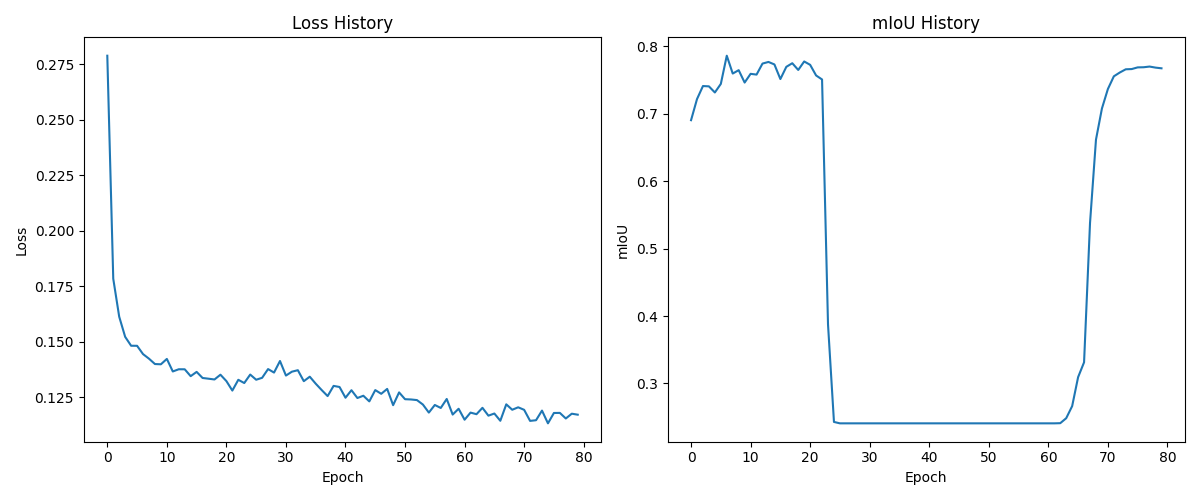
\includegraphics[width=\textwidth]{test2/metrics.png}
        \caption{Niestabilność gradientu (Test 2) -- widoczny brak postępu w~fazie początkowej oraz oscylacje metryk.}
        \label{fig:dyn_a}
    \end{subfigure}
    \\[0.5cm]
    \begin{subfigure}[b]{0.85\textwidth}
        \centering
        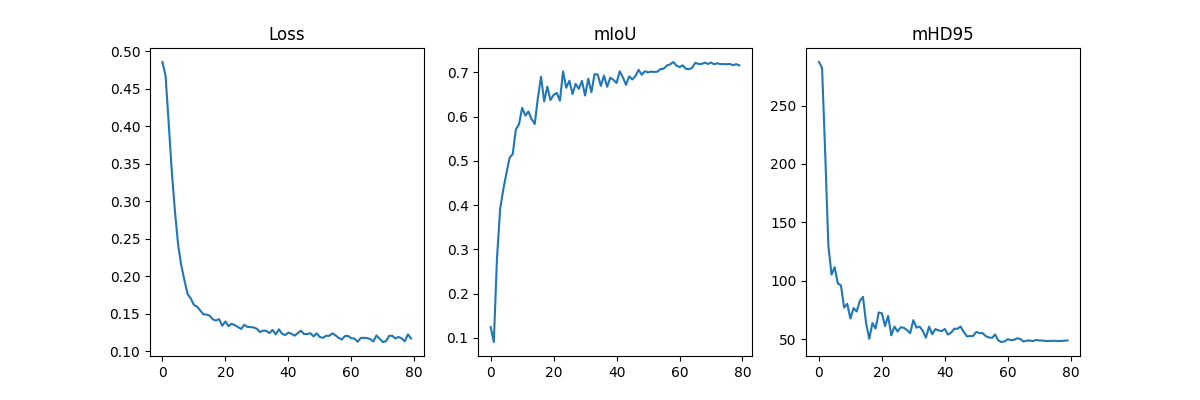
\includegraphics[width=\textwidth]{test18/metrics.png}
        \caption{Stabilny proces uczenia (Test 18) -- harmonijny przebieg optymalizacji dzięki zastosowaniu mechanizmu rozgrzewki.}
        \label{fig:dyn_b}
    \end{subfigure}
    \caption{Dynamika procesu uczenia: (a) przypadek z~niestabilnym gradientem oraz (b) proces zoptymalizowany z~wykorzystaniem mechanizmu \textit{warmup}.}
    \label{fig:training_dynamics}

\end{figure}
\subsection{Skalowanie architektury a~generalizacja}
Przejście z~enkodera MiT-B2 na MiT-B3 (44~mln parametrów) w~Teście 10 wykazało, że dla specyfiki zbioru RETOUCH większa pojemność modelu prowadzi do szybkiego przeuczenia (\textit{overfittingu}). Skutkowało to spadkiem metryk na zbiorze walidacyjnym o~ponad 5\% względem modelu lżejszego. Optymalnym rozwiązaniem okazała się architektura \textbf{SegFormer-B2}.

\subsection{Zbiorcze zestawienie wyników ilościowych}
Zestawienie kluczowych eksperymentów przedstawiono w~tabeli~\ref{tab:results_all}. Model optymalny wykorzystuje kontekst 2.5D oraz funkcję kosztu Tversky Loss.
\begin{table}[htbp]
    \centering
    \small
    \caption{Rozszerzone zestawienie wyników dla wszystkich eksperymentów zespołów CNN i~Transformers.}
    \label{tab:results_all}
    \begin{tabularx}{\textwidth}{lXcc}
        \toprule
        Metoda & Opis szczegółowy & mIoU & mDice \\
        \midrule
        \textbf{Zbiór CNN} & & & \\
        \textbf{U-Net ResNet34} & \textbf{wagi dynamiczne, clahe,tta} & \textbf{0,7446} & \textbf{0,8459} \\
        U-Net ResNet34 & clahe,tta & 0,7375 & 0,8406 \\
        ResNet34 & Baseline & 0,7166 & 0,8235 \\
        Attention U-Net 2D & Rozdzielczość 1024 px & 0,6718 & 0,7906 \\
        Attention U-Net 2.5D & Kontekst 3-kanałowy & 0,6627 & 0,7838 \\
        Attention U-Net 2D & MRS 20 + CLAHE & 0,6336 & 0,7590 \\
        Attention U-Net 2D & Konfiguracja MRS 0 & 0,5694 & 0,6973 \\
        nnU-Net 2D & Baseline referencyjny & 0.7141 & 0.8332 \\
        \midrule
        \textbf{Zbiór Transformers} & & & \\
        \textbf{SegFormer-B2} & \textbf{Kontekst 2.5D, Tversky (Model optymalny)} & \textbf{0,7529} & \textbf{0,8521} \\
        \textbf{SegFormer-B2} & \textbf{High-Recall Tuning (Test 18)} & \textbf{0,6990} & \textbf{0,8118} \\
        SegFormer-B2 & Edge Awareness (Test 14) & 0,7405 & 0,8431 \\
        SegFormer-B2 & 2.5D + Boundary Loss (Test 13) & 0,7186 & 0,8273 \\
        SegFormer-B2 & Single-slice Baseline (Test 9) & 0,7409 & 0,8434 \\
        SegFormer-B3 & Skalowanie (Overfitting, Test 10) & 0,6844 & 0,8014 \\
        \bottomrule
    \end{tabularx}
\end{table}

\subsection{Analiza kompromisu: Stabilność vs Czułość Kliniczna}
Porównanie modelu optymalnego z~modelem wysokiej czułości (Test 18) przedstawiono w~tabeli~\ref{tab:test11_vs_test18}. Spadek metryk geometrycznych (DSC, IoU) w~wariancie High-Recall wynika z~agresywnej optymalizacji pod kątem wykrywania wszystkich zmian patologicznych (minimalizacja FN). Dla klinicysty okulisty, wyższa czułość detekcji małych cyst jest priorytetem, nawet kosztem lekkiego przeszacowania ich obrysów.

\begin{table}[htbp]
 \centering
 \caption{Analiza wpływu optymalizacji \textit{High-Recall} na metryki segmentacji.}
 \label{tab:test11_vs_test18}
 \begin{tabular}{lccc}
 \toprule
 Metryka & Model optymalny & Model High-Recall & Różnica \\
 \midrule
 mIoU & \textbf{0,7529} & 0,6990 & -0,0539 \\
 mDice & \textbf{0,8521} & 0,8118 & -0,0403 \\
 mHD95 [px] & \textbf{67,31} & 74,84 & +7,53 \\
 \midrule
 IRF Dice (Klasa 1) & \textbf{0,7483} & 0,6800 & -0,0683 \\
 SRF Dice (Klasa 2) & \textbf{0,8489} & 0,8187 & -0,0302 \\
 PED Dice (Klasa 3) & \textbf{0,8220} & 0,7634 & -0,0586 \\
 \bottomrule
 \end{tabular}
\end{table}

\section{Charakterystyka parametrów modeli}

Ważnym aspektem praktycznego wdrożenia systemów głębokiego uczenia jest ich złożoność obliczeniowa, mierzona liczbą parametrów uczonych. Zestawienie dla kluczowych architektur przedstawiono w~tabeli~\ref{tab:performance_stats}. 

\begin{table}[htbp]
    \centering
    \caption{Zestawienie liczby parametrów analizowanych architektur.}
    \label{tab:performance_stats}
    \begin{tabular}{lc}
        \toprule
        Model & Liczba parametrów [mln] \\
        \midrule
        SegFormer-B2 (Model optymalny) & 27,35 \\
        U-Net ResNet34 & 24,44 \\
        nnU-Net 2D (Baseline) & 31,17 \\
        \bottomrule
    \end{tabular}
\end{table}

Precyzyjne pomiary czasu wnioskowania (\textit{inference time}) dla pojedynczych przekrojów oraz szczegółowe benchmarki obciążenia pamięci VRAM w~warunkach operacyjnych nie zostały ujęte w~niniejszym raporcie. Pełna analiza wydajnościowa, obejmująca porównanie prędkości działania na GPU oraz optymalizację zużycia zasobów zarówno dla modeli transformerowych, jak i~systemu nnU-Net, stanowi kierunek dalszych prac badawczych zaplanowanych na okres wakacyjny.

\chapter{Analiza jakościowa i~dyskusja}

\section{Interpretacja wyników w~kontekście klinicznym}
Osiągnięte wyniki potwierdzają, że nowoczesne architektury transformerowe wykazują wysoką zdolność do modelowania złożonej morfologii patologii siatkówki. Uzyskana wartość współczynnika mDice dla modelu optymalnego (0,8521) świadczy o~wysokiej wiarygodności automatycznej segmentacji, co w~warunkach klinicznych może znacząco skrócić czas analizy wolumenów OCT przez lekarzy okulistów.

\section{Analiza porażek i~konflikt sygnałów przestrzennych}

Eksperyment nr 13 (\textit{The Grand Synthesis}) dostarczył kluczowej wiedzy o~granicach hybrydyzacji metod. Próba jednoczesnego zastosowania kontekstu 2.5D oraz funkcji \textit{Boundary Loss} przyniosła niespodziewaną regresję wyników.

Analiza logów wykazała fundamentalny konflikt: kontekst 2.5D, agregując informację z~trzech sąsiednich skanów, wprowadza naturalne wygładzenie sygnału przestrzennego. Z~kolei \textit{Boundary Loss}, oparty na dystansie euklidesowym od krawędzi, wymaga skrajnej ostrości granic do poprawnego wyznaczania gradientów. W~wyniku nałożenia tych mechanizmów doszło do destabilizacji granic segmentacji na obrazach o~wysokim zaszumieniu typu \textit{speckle}, co potwierdził wzrost metryki HD95.

\section{Wpływ kontekstu 2.5D na spójność wolumetryczną}
Analiza wizualna predykcji potwierdziła, że wprowadzenie logiki 2.5D (Test 12) kluczowo wpłynęło na redukcję fałszywych detekcji. Dzięki dostarczeniu modelowi informacji o~sąsiednich przekrojach, sieć zyskała zdolność do weryfikacji ciągłości struktur płynowych. Pozwoliło to na skuteczną eliminację izolowanych błędów segmentacji pojawiających się w~ciele szklistym, które w~modelach typu \textit{single-slice} były mylnie klasyfikowane jako płyn podsiatkówkowy (SRF).

\section{Dyskusja o~kompromisie: Model optymalny vs High-Recall}
Wyniki Testu 18 dostarczają istotnych przesłanek do dyskusji o~praktycznym zastosowaniu AI w~medycynie. Zaobserwowany spadek metryk Dice i~IoU nie jest wynikiem degradacji jakości modelu, lecz świadomego przesunięcia punktu pracy w~stronę wyższej czułości (\textit{Recall}). W~diagnostyce medycznej pominięcie zmiany patologicznej (błąd II rodzaju) jest znacznie bardziej kosztowne niż fałszywy alarm. Model High-Recall, dzięki agresywnemu strojeniu funkcji Tversky ($\alpha=0.1, \beta=0.9$), minimalizuje ryzyko utraty informacji o~początkowych stadiach obrzęku.

\section{Analiza wizualna mechanizmów uwagi (Attention Maps)}
W~celu empirycznej weryfikacji procesu podejmowania decyzji przez model SegFormer, przeprowadzono ekstrakcję wag atencji z~poszczególnych etapów enkodera MiT. 

\subsection{Płyn podsiatkówkowy (SRF) i~odwarstwienie nabłonka (PED)}
W~przypadku klas SRF oraz PED, mechanizm uwagi wykazał się wysoką precyzją. Jak przedstawiono na rysunkach~\ref{fig:attention_srf_all} oraz~\ref{fig:attention_ped_all}, na etapach 6 i~7 model generuje wyraźne aktywacje koncentrujące się bezpośrednio na granicach patologii oraz na warstwie nabłonka barwnikowego siatkówki (RPE). Świadczy to o~zdolności transformera do poprawnego rozpoznania globalnej topologii siatkówki.

\subsection{Wyzwania w~segmentacji drobnych cyst IRF}
Zaobserwowano, że dla klasy IRF (Rysunek~\ref{fig:attention_irf_all}) mapy atencji na głębszych poziomach są znacznie bardziej rozproszone i~trudne w~interpretacji. Wynika to z~faktu, że mikroskopijne cysty IRF zajmują zbyt małą powierzchnię w~stosunku do szerokiego pola widzenia głębokich warstw transformera. Sygnał uwagi ulega w~takim przypadku uśrednieniu, co potwierdza, że segmentacja IRF opiera się w~większym stopniu na cechach lokalnych przekazywanych przez hierarchiczną strukturę enkodera niż na globalnych zależnościach kontekstowych.

\begin{figure}[htbp]
    \centering
    \begin{subfigure}[b]{0.23\textwidth}
        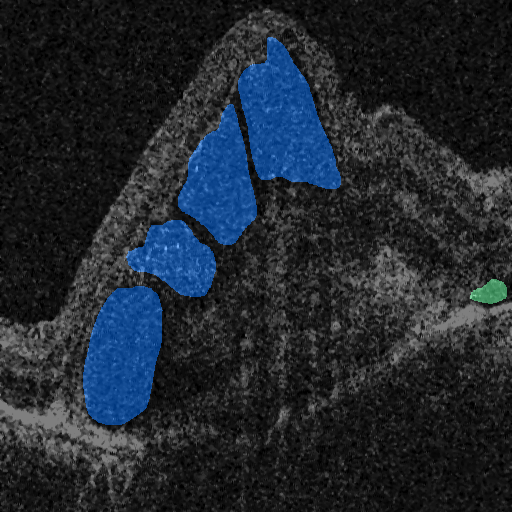
\includegraphics[width=\textwidth]{test18/attention_maps/att_idx331_IRF_GT_OVERLAY.png}
        \caption{IRF: GT Overlay}
    \end{subfigure}
    \hfill
    \begin{subfigure}[b]{0.23\textwidth}
        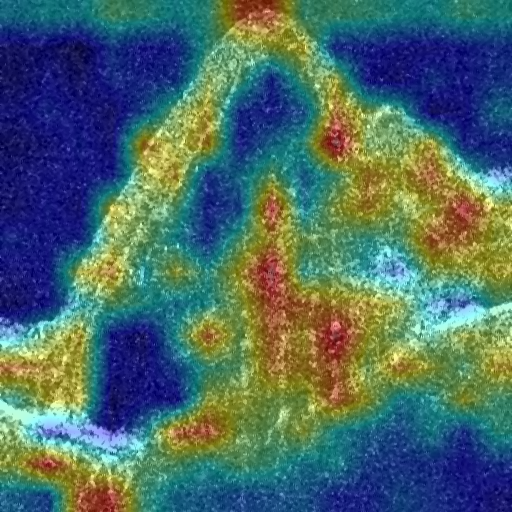
\includegraphics[width=\textwidth]{test18/attention_maps/att_idx331_IRF_stage0.png}
        \caption{IRF: Stage 0}
    \end{subfigure}
    \hfill
    \begin{subfigure}[b]{0.23\textwidth}
        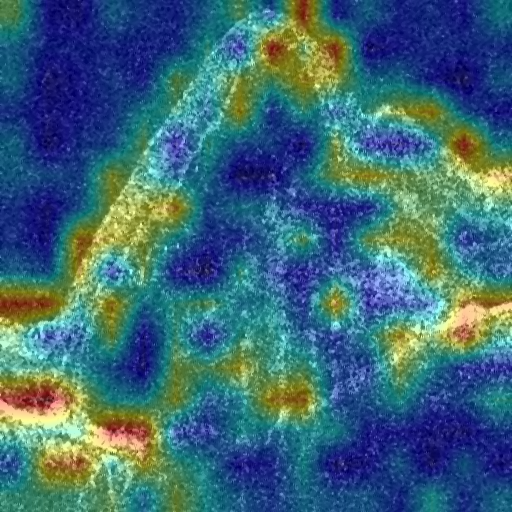
\includegraphics[width=\textwidth]{test18/attention_maps/att_idx331_IRF_stage6.png}
        \caption{IRF: Stage 6}
    \end{subfigure}
    \hfill
    \begin{subfigure}[b]{0.23\textwidth}
        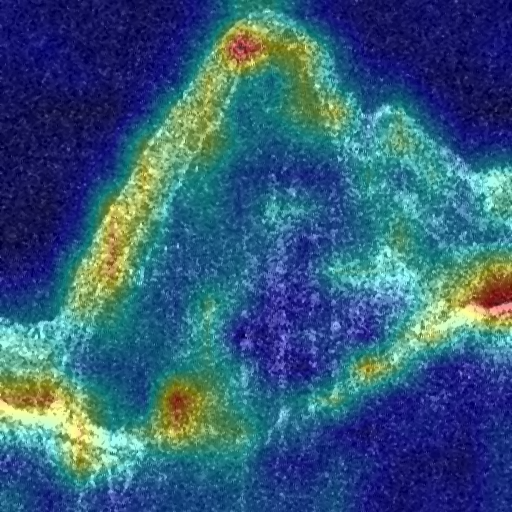
\includegraphics[width=\textwidth]{test18/attention_maps/att_idx331_IRF_stage11.png}
        \caption{IRF: Stage 11}
    \end{subfigure}
    \caption{Wizualizacja mechanizmu uwagi dla płynu wewnątrzsiatkówkowego (IRF) -- przypadek 331. Widoczne rozproszenie sygnału uwagi na głębszych poziomach.}
    \label{fig:attention_irf_all}
\end{figure}

\begin{figure}[htbp]
    \centering
    \begin{subfigure}[b]{0.23\textwidth}
        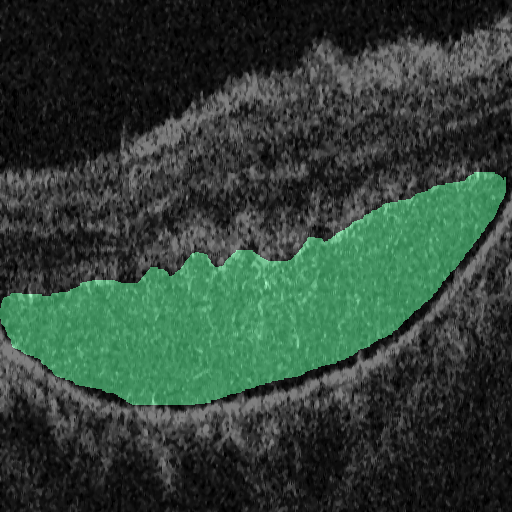
\includegraphics[width=\textwidth]{test18/attention_maps/att_idx283_SRF_GT_OVERLAY.png}
        \caption{SRF: GT Overlay}
    \end{subfigure}
    \hfill
    \begin{subfigure}[b]{0.23\textwidth}
        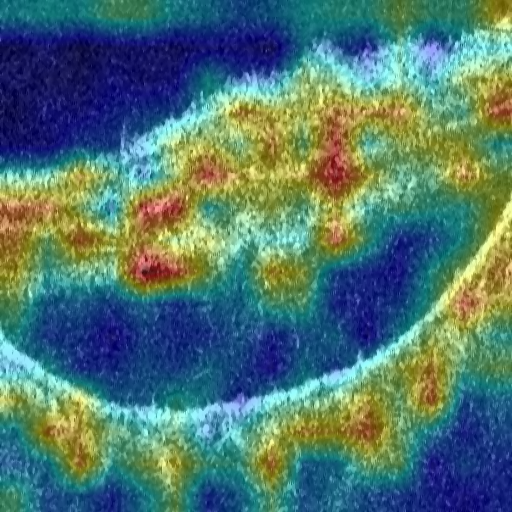
\includegraphics[width=\textwidth]{test18/attention_maps/att_idx283_SRF_stage0.png}
        \caption{SRF: Stage 0}
    \end{subfigure}
    \hfill
    \begin{subfigure}[b]{0.23\textwidth}
        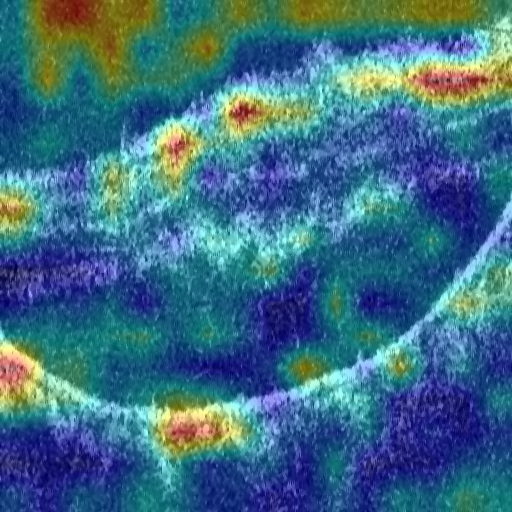
\includegraphics[width=\textwidth]{test18/attention_maps/att_idx283_SRF_stage3.png}
        \caption{SRF: Stage 3}
    \end{subfigure}
    \hfill
    \begin{subfigure}[b]{0.23\textwidth}
        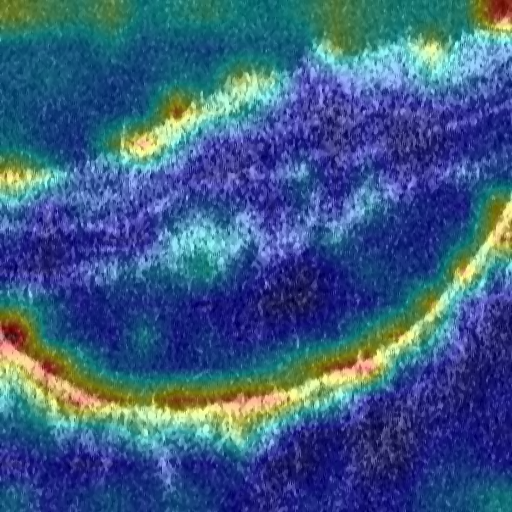
\includegraphics[width=\textwidth]{test18/attention_maps/att_idx283_SRF_stage7.png}
        \caption{SRF: Stage 7}
    \end{subfigure}
    \caption{Mapy atencji dla płynu podsiatkówkowego (SRF) -- przypadek 283. Precyzyjna lokalizacja granic patologii na etapie 7.}
    \label{fig:attention_srf_all}
\end{figure}

\begin{figure}[htbp]
    \centering
    \begin{subfigure}[b]{0.23\textwidth}
        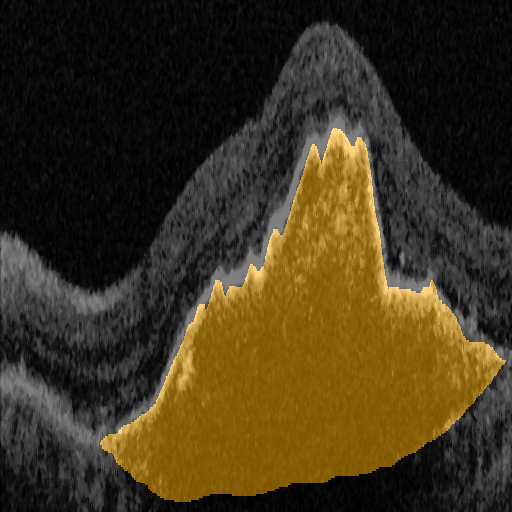
\includegraphics[width=\textwidth]{test18/attention_maps/att_idx556_PED_GT_OVERLAY.png}
        \caption{PED: GT Overlay}
    \end{subfigure}
    \hfill
    \begin{subfigure}[b]{0.23\textwidth}
        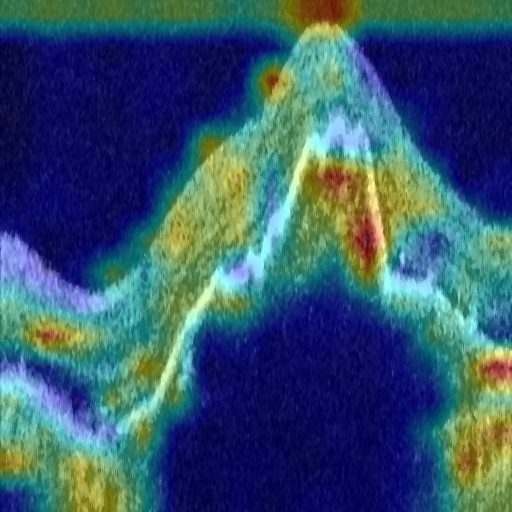
\includegraphics[width=\textwidth]{test18/attention_maps/att_idx556_PED_stage0.png}
        \caption{PED: Stage 0}
    \end{subfigure}
    \hfill
    \begin{subfigure}[b]{0.23\textwidth}
        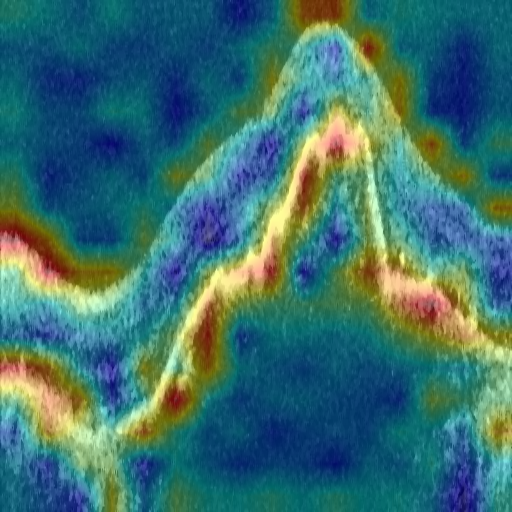
\includegraphics[width=\textwidth]{test18/attention_maps/att_idx556_PED_stage6.png}
        \caption{PED: Stage 6}
    \end{subfigure}
    \hfill
    \begin{subfigure}[b]{0.23\textwidth}
        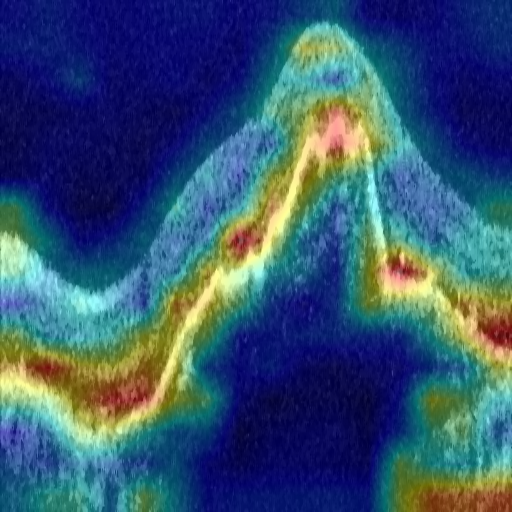
\includegraphics[width=\textwidth]{test18/attention_maps/att_idx556_PED_stage11.png}
        \caption{PED: Stage 11}
    \end{subfigure}
    \caption{Wizualizacja mechanizmu uwagi dla odwarstwienia nabłonka barwnikowego siatkówki (PED) -- przypadek 556.}
    \label{fig:attention_ped_all}
\end{figure}

\chapter{Podsumowanie i~wnioski}

\section{Realizacja celu pracy}

Głównym celem niniejszej pracy było opracowanie i~porównanie skuteczności nowoczesnych architektur transformerowych w~zadaniu automatycznej, wieloklasowej segmentacji patologicznych przestrzeni płynowych (IRF, SRF, PED) na obrazach OCT.\@ Cel ten został zrealizowany poprzez implementację modeli SegFormer oraz wstępną walidację architektury SwinUNETR na standaryzowanym zbiorze danych RETOUCH.\@ Przeprowadzone badania wykazały, że modele oparte na mechanizmie uwagi stanowią wydajną alternatywę dla klasycznych sieci konwolucyjnych (CNN), oferując nie tylko wysoką precyzję ilościową, ale również nową jakość w~postaci interpretowalnych map atencji.

\section{Wnioski końcowe}

Na podstawie przeprowadzonych eksperymentów sformułowano następujące wnioski:
\begin{enumerate}
 \item \textbf{Efektywność kontekstu przestrzennego:} Zastosowanie podejścia 2.5D znacząco poprawiło wyniki segmentacji, szczególnie w~przypadku płynu podsiatkówkowego (SRF), poprzez wykorzystanie informacji o~ciągłości struktur w~przestrzeni wolumetrycznej.
 \item \textbf{Optymalna skala architektury:} Dla analizowanego wolumenu danych treningowych rozwiązaniem optymalnym okazał się model SegFormer-B2. Wykazano, że dalsze zwiększanie liczby parametrów (skalowanie do B3) prowadzi do szybkiego przeuczenia modelu bez wymiernych korzyści dla precyzji segmentacji.
 \item \textbf{Wartość kliniczna interpretowalności:} Analiza map atencji dla warstw 6 i~7 potwierdziła, że model poprawnie identyfikuje kluczowe biomarkery strukturalne (RPE, PED). Jednocześnie wykazano ograniczenia globalnego mechanizmu uwagi w~detekcji mikroskopijnych cyst IRF, co wyznacza granicę ufności wobec map atencji na tym poziomie hierarchii.
\end{enumerate}

\section{Potencjalne kierunki dalszych prac}

Realizacja raportu częściowego pozwoliła na zidentyfikowanie kluczowych obszarów rozwoju systemu:
\begin{itemize}
 \item \textbf{Ekspansja bazy danych:} Głównym ograniczeniem obecnych modeli jest relatywnie mały zbiór danych treningowych. Planowane na okres wakacyjny pozyskanie nowych wolumenów OCT pozwoli na pełne wykorzystanie potencjału głębokich Transformerów.
 \item \textbf{Pełne przetwarzanie 3D:} Optymalizacja zużycia zasobów obliczeniowych modelu SwinUNETR 3D w~celu przejścia z~reprezentacji 2.5D na natywne przetwarzanie wolumetryczne.
 \item \textbf{Hybrydowe systemy eksperckie (Test 19):} Wdrożenie architektury typu \textit{Ensemble}, w~której obok modelu bazowego pracować będzie wyspecjalizowany, lekki model binarny (tzw.~\textit{IRF Expert}). Takie podejście ma na celu przełamanie barier w~precyzyjnej detekcji drobnych, rozproszonych cyst IRF przy jednoczesnym zachowaniu wysokiej czułości klinicznej.
\end{itemize}

\bibliographystyle{plainnat}
\bibliography{bibliografia}

\end{document}
